\chapter{\ifproject%
\ifenglish Project Structure and Methodology\else โครงสร้างและขั้นตอนการทำงาน\fi
\else%
\ifenglish Project Structure\else โครงสร้างของโครงงาน\fi
\fi
}

\makeatletter

% \renewcommand\section{\@startsection {section}{1}{\z@}%
%                                    {13.5ex \@plus -1ex \@minus -.2ex}%
%                                    {2.3ex \@plus.2ex}%
%                                    {\normalfont\large\bfseries}}

\makeatother
%\vspace{2ex}
% \titleformat{\section}{\normalfont\bfseries}{\thesection}{1em}{}
% \titlespacing*{\section}{0pt}{10ex}{0pt}

\section{สถาปัตยกรรมระบบ}
  \qquad โครงงานนี้ได้ออกแบบสถาปัตยกรรมของระบบเป็นแบบ \textbf{Microservices} โดยบทนี้จะกล่าวถึง
    โครงสร้างของระบบทั้งหมด และอธิบายถึงแต่ละส่วนของระบบ โดยระบบจะถูกแบ่งออกเป็นส่วนย่อยๆ 
    แต่ละส่วนจะมีหน้าที่และความรับผิดชอบในการทำงานที่แตกต่างกัน

    \begin{figure}[!ht]
      \centering
      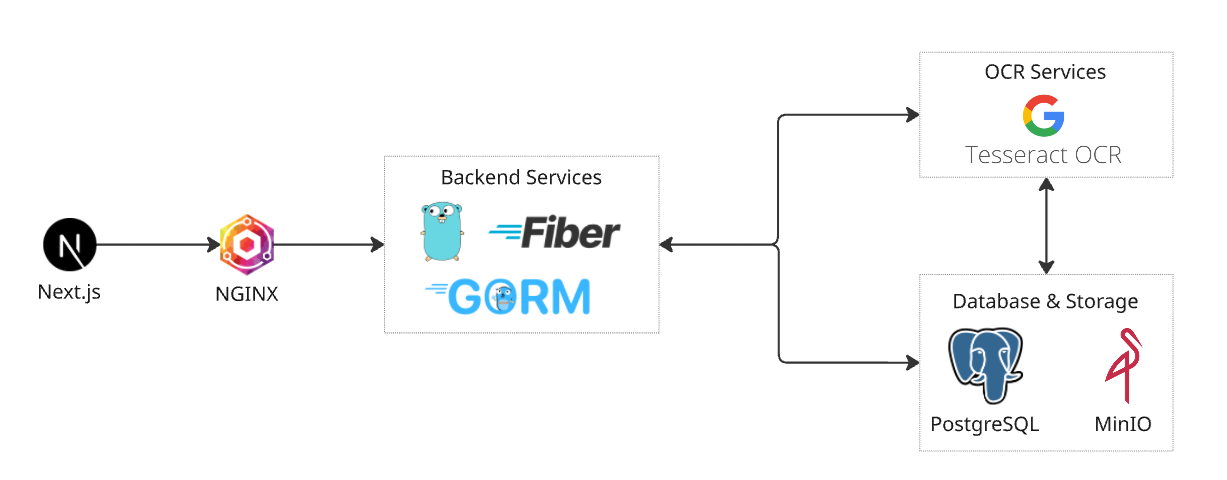
\includegraphics[width=0.8\textwidth]{image/Approach/Architecture.png}
      \caption[Architecture]{System Architecture}
      \label{fig:architecture}
    \end{figure}
    \FloatBarrier

  จากรูปที่ 3.1 แสดงถึงสถาปัตยกรรมของระบบที่ถูกแบ่งออกเป็นส่วนย่อยๆ ดังนี้
  \begin{enumerate}
    \item \textbf{Frontend} ส่วนนี้เป็นส่วนที่ทำหน้าที่ในการแสดงผลของระบบ โดยส่วนนี้จะถูกพัฒนาด้วย \textbf{Next.js}
    \item \textbf{Reverse Proxy} ส่วนนี้เป็นส่วนที่ทำหน้าที่ในการจัดการการเชื่อมต่อระหว่าง Frontend และ Backend
    โดยส่วนนั้นจะถูกพัฒนาด้วย \textbf{Nginx Proxy Manager(NPM)}
    \item \textbf{Backend} ส่วนนี้เป็นส่วนที่ทำหน้าที่ในการประมวลผลข้อมูลและให้บริการ API โดยส่วนนั้นจะถูกพัฒนาด้วย
    \textbf{Go (Golang)} และเฟรมเวิร์ก \textbf{Fiber}
    \item \textbf{OCR Service} ส่วนนี้เป็นส่วนที่ทำหน้าที่ในการประมวลผลภาพและทำการรู้จำตัวอักษร โดยส่วนนั้นจะถูกพัฒนาด้วย \textbf{Tesseract OCR}
    \item \textbf{Database and Storage} ส่วนนี้เป็นส่วนที่ทำหน้าที่ในการจัดเก็บข้อมูล โดยจะใช้ \textbf{PostgreSQL}
    เป็นฐานข้อมูลหลัก และใช้ \textbf{MinIO} สำหรับการจัดเก็บไฟล์
  \end{enumerate}

\section{โครงสร้างฐานข้อมูล (Database Schema)}
  \begin{figure}[!ht]
    \centering
    \includegraphics[width=1\textwidth]{image/Approach/Database-Schema.png}
    \caption[Database Schema]{Database Schema}
    \label{fig:database_schema}
  \end{figure}
  \FloatBarrier
  \qquad ฐานข้อมูลที่ใช้ในโครงงานนี้ คือ PostgreSQL โดยมีการออกแบบโครงสร้างฐานข้อมูล (Database Schema) เพื่อรองรับการทำงานของแพลตฟอร์มอย่างมีประสิทธิภาพ
  โดยโครงสร้างฐานข้อมูลประกอบด้วยตารางหลักๆ ดังนี้
  \begin{enumerate}
    \item \textbf{Universities} ตารางสำหรับเก็บข้อมูลรายการมหาวิทยาลัย
    \item \textbf{User Groups} ตารางสำหรับเก็บข้อมูลประเภทกลุ่มของผู้ใช้งานในแพลตฟอร์ม
    \item \textbf{Users} ตารางสำหรับเก็บข้อมูลต่างๆ ของผู้ใช้งานในแพลตฟอร์ม
    \item \textbf{Courses} ตารางสำหรับเก็บข้อมูลกระบวนวิชา
    \item \textbf{Sections} ตารางสำหรับเก็บข้อมูลลำดับตอนภายในกระบวนวิชา
    \item \textbf{Enrollment lists} ตารางสำหรับเก็บข้อมูลการลงทะเบียนของผู้ใช้งานในกระบวนวิชา
    \item \textbf{Personal Data} ตารางสำหรับเก็บข้อมูลของผู้ใช้งานในกระบวนวิชาที่ได้ลงทะเบียน
    \item \textbf{Assignments} ตารางสำหรับเก็บข้อมูลการมอบหมายงาน
    \item \textbf{Assignment Files} ตารางสำหรับเก็บข้อมูลไฟล์การมอบหมายงาน
    \item \textbf{Assignment Sections} ตารางสำหรับเก็บข้อมูลลำดับตอนภายในการมอบหมายงาน
    \item \textbf{Export Grades} ตารางสำหรับเก็บข้อมูลการส่งออกเกรด
    \item \textbf{Rubrics} ตารางสำหรับเก็บข้อมูลเกณฑ์การประเมินของใบงาน
    \item \textbf{Bounding Boxes} ตารางสำหรับเก็บข้อมูลกรอบของแต่ละใบงาน
    \item \textbf{Submissions} ตารางสำหรับเก็บข้อมูลการส่งใบงาน หรืออัพโหลดใบงาน
    \item \textbf{Submission Boxes} ตารางสำหรับเก็บข้อมูลกล่องของแต่ใบงาน ที่ใช้ในการทำ Optical Character Recognition (OCR)
    \item \textbf{Uploads} ตารางสำหรับเก็บข้อมูลการอัปโหลดไฟล์ใบงาน
    \item \textbf{Grades} ตารางสำหรับเก็บข้อมูลการให้คะแนน
  \end{enumerate}

\section{โครงสร้างระบบจัดเก็บข้อมูลแบบอ็อบเจ็กต์ (Object Storage)}
  \qquad โครงสร้างระบบจัดเก็บข้อมูลแบบอ็อบเจ็กต์ (Object Storage) ที่ใช้ในโครงงานนี้ คือ MinIO โดยมีการออกแบบโครงสร้างเพื่อรองรับการจัดเก็บไฟล์ต่างๆ
  ที่เกี่ยวข้องกับการทำงานของแพลตฟอร์ม โดยทางผู้พัฒนาได้ออกแบบไว้ในรูปแบบของ Bucket ดังนี้
  \subsection{Buckets} เป็นโครงสร้างหลักที่ใช้ในการจัดเก็บข้อมูลไฟล์ต่างๆ โดยในโครงงานนี้ได้สร้าง Bucket หลักๆ ดังนี้
    \begin{enumerate}
      \item 
      \item 
      \item 
      \item 
    \end{enumerate}

\section{Frontend}
  \qquad Frontend เป็นส่วนที่ผู้ใช้จะโต้ตอบด้วยผ่านทางเว็บเบราว์เซอร์ โดยมีหน้าที่หลักในการแสดงผลข้อมูลและรับคำสั่งจากผู้ใช้
  ซึ่งในโครงงานนี้ได้ใช้ Next.js เป็นเฟรมเวิร์กหลักในการพัฒนา และใช้ Tailwind CSS ร่วมกับ MantineUI ในการออกแบบส่วนติดต่อผู้ใช้ (User Interface)

  \section{การใช้งานพื้นฐาน}
    \qquad แพลตฟอร์มนี้ถูกออกแบบมาให้มี User Interface สำหรับผู้ใช้งาน 2 ประเภท ได้แก่ ผู้สอน (Instructor) และนักศึกษา (Student) โดยแต่ละประเภทจะมีหน้าที่และการใช้งานที่แตกต่างกัน ดังนี้
  \subsection{ผู้สอน (Instructor)}
    \par\hspace*{3em} ผู้สอนมีหน้าที่ในการสร้างคอร์สและมอบหมายงานให้กับนักศึกษา รวมถึงการตรวจสอบและให้คะแนนงานที่นักศึกษาส่งมา 
    \begin{enumerate}
        \item Courses Overview ส่วนนี้เป็นส่วนที่ทําหน้าที่ในการแสดงผลหน้าแรกของเว็บไซต์หลังทําการ Login เข้าสู่ระบบ
        \item Dashboard ส่วนนี้เป็นส่วนที่ทําหน้าที่ในการแสดงผลภาพรวมของคอร์สที่ผู้สอนได้สร้างขึ้น
        \item Assignments Management ส่วนนี้เป็นส่วนที่ทําหน้าที่ในการจัดการงานที่ผู้สอนได้มอบหมายให้กับนักศึกษา
        \item Roster Management ส่วนนี้เป็นส่วนที่ทําหน้าที่ในการจัดการรายชื่อนักศึกษาที่ลงทะเบียนในคอร์ส
        \item Export Grades ส่วนนี้เป็นส่วนที่ทําหน้าที่ในการส่งออกข้อมูลงานที่ได้รับหมอบหมายเป็นไฟล์ CSV 
        \item Edit Outline ส่วนนี้เป็นส่วนที่ทําหน้าที่ในการสร้างโครงร่างของงานที่ผู้สอนจะใช้ในการตรวจ
        \item Manage Submissions ส่วนนี้เป็นส่วนที่ทําหน้าที่ในการจัดการจับคู่ใบงานที่ผู้สอนเป็นผู้อัพโหลด
        \item Grade Submissions ส่วนนี้เป็นส่วนที่ทําหน้าที่ในการให้คะแนนงานทีได้หมอบหมายให้กับนักศึกษา
        \item Review Grades ส่วนนี้เป็นส่วนที่ทำหน้าที่แสดงสถิติของงานที่ได้รับหมอบหมายพร้อมรายชื่อของนักศึกษาที่ส่งงาน
        \item statistics ส่วนนี้เป็นส่วนที่ทําหน้าที่ในการแสดงผลสถิติของงานที่ได้รับหมอบหมาย 
    \end{enumerate}
  \subsection{นักศึกษา (Student)}
    \par\hspace*{3em} นักศึกษามีหน้าที่ในการตรวจสอบและส่งงานที่ได้รับมอบหมาย
    \begin{enumerate}
        \item Dashboard ส่วนนี้เป็นส่วนที่ทําหน้าที่ในการแสดงผลภาพรวมของงานที่นักศึกษาได้รับหมอบหมายไว้
        \item Courses Overview ส่วนนี้เป็นส่วนที่ทําหน้าที่ในการแสดงผลภาพรวมของคอร์สที่นักศึกษาได้อยู่ในระบบ
        \item Course Dashboard ส่วนนี้เป็นส่วนที่ทําหน้าที่ในการแสดงผลรายละเอียดของคอร์สที่นักศึกษาได้ลงทะเบียนไว้
    \end{enumerate}
